\documentclass[20pt, a1paper, portrait, margin=0mm, innermargin=10mm,
     blockverticalspace=8mm, colspace=10mm, subcolspace=8mm]{tikzposter}

\usepackage{amssymb,amsmath}
\usepackage{mathtools}

\usepackage{amsthm}
\newtheoremstyle{break}
  {\topsep}{\topsep}%
  {\itshape}{}%
  {\bfseries}{}%
  {\newline}{}%
\theoremstyle{break}
\newtheorem*{Theorem}{Theorem}
\newtheorem*{Definition}{Definition}

\usepackage{graphicx}
\usepackage{xcolor}
\usepackage{adjustbox}
\usepackage{tikz}
\usepackage[none]{hyphenat}

\usetikzlibrary{automata,arrows,positioning}

% Orange brand colours
% core colours
\definecolor{brand-orange}{RGB}{255,121,0}
% support colours
\definecolor{brand-blue}{RGB}{75,180,230}
% functional greys
\definecolor{brand-lightgrey}{RGB}{246,246,246}
% functional colours
\definecolor{brand-func-blue}{RGB}{82,126,219}

\usetikzlibrary{arrows.meta}
\tikzset{>={Latex[width=4mm,length=4mm]}}
\tikzstyle{switch-style}=[circle, draw, thin, fill=brand-blue, scale=0.3]
\tikzstyle{controller-style}=[rectangle, thin, fill=brand-orange, scale=0.8]
\tikzstyle{rpath}=[ultra thick, brand-orange, opacity=0.4]
\tikzstyle{rounded-box}=[rectangle, rounded corners, draw=black, very thick, minimum height=2em, text centered]

\title{{\bf Epidemic Control with Learning \& Optimization}}
\author{{\bf Paul Beaujean$^{\dagger *}$\\
{\Large \textbf{Advisors:} Prof. Cristina Bazgan$^{\dagger}$, \'Eric
Gourdin$^{*}$}}}
\institute{{\large
$^{\dagger}$LAMSADE, Universit\'e Paris-Dauphine, $^{*}$Orange Labs}}
\titlegraphic{
    \includegraphics[scale=0.27]{logo_cnrs}
        \qquad\qquad\qquad
    
\includegraphics[scale=0.4]{logo_dauphine}
        \qquad\qquad\qquad
    
\includegraphics[scale=1.5]{logo_lamsade}
        \qquad\qquad\qquad
    
\includegraphics[scale=0.3]{logo_cmyk}
}

% Choose LAYOUT:  Default, Basic, Rays, Simple, Envelope, Wave, Board, Autumn, Desert,
\usetheme{Autumn}
\definecolorstyle{myColorStyle}{
\colorlet{colorOne}{black}
\colorlet{colorTwo}{white}
\colorlet{colorThree}{brand-blue}
}{
% Background Colors
\colorlet{backgroundcolor}{brand-blue}
\colorlet{framecolor}{black}
% Title Colors
\colorlet{titlefgcolor}{brand-blue}
\colorlet{titlebgcolor}{white}
% Block Colors
\colorlet{blocktitlebgcolor}{white}
\colorlet{blocktitlefgcolor}{brand-blue}
\colorlet{blockbodybgcolor}{white}
\colorlet{blockbodyfgcolor}{black}
% Innerblock Colors
\colorlet{innerblocktitlebgcolor}{white}
\colorlet{innerblocktitlefgcolor}{black}
\colorlet{innerblockbodybgcolor}{white}
\colorlet{innerblockbodyfgcolor}{black}
% Note colors
\colorlet{notefgcolor}{black}
\colorlet{notebgcolor}{white}
\colorlet{notefrcolor}{white}
}
%Default, Australia, Britain, Sweden, Spain, Russia, Denmark, Germany
\usecolorstyle[colorOne=black, colorTwo=brand-blue,
colorThree=brand-blue]{myColorStyle}
\usetitlestyle[titletoblockverticalspace=10mm]{Filled}

\begin{document}
\maketitle{}

\begin{columns}
  \column{0.4}
  \block{Network security}{
    \begin{itemize}
      \item[$\circ$] Networked systems face propagation of malware, cascading
	hardware failures, DDoS.
      \item[$\circ$] Software-defined networking enables full automated control
	over network topology.
    \end{itemize}
    \begin{tikzfigure}
      \begin{tikzpicture}[auto, thick]
       % Cloud creation
       \node[cloud, fill=brand-lightgrey, cloud puffs=16, cloud puff arc= 100,
	minimum width=7cm, minimum height=2.5cm, aspect=1] (cloud) at (0,0) {};
	\node (cloud-legend)[right=0.5cm of cloud] {Logical Topology};

       % Physical layer nodes
	\foreach \place/\x in {{(-2.5,0.3)/1}, {(-1.75,-0.55)/2},{(-1.2,0.55)/3},
	  {(-0.75,-0.7)/4}, {(-0.25,0)/5}, {(0.25,0.7)/6}, {(0.75,-0.3)/7},
	  {(1.5,0)/8},{(2.5,0.4)/9}}
	\node[switch-style] (a\x) at \place {};

	% SDN topology links
	\path[thin] (a1) edge (a2);
	\path[thin] (a1) edge (a3);
	\path[thin] (a2) edge (a3);
	\path[thin] (a3) edge (a6);
	\path[thin] (a2) edge (a4);
	\path[thin] (a5) edge (a6);
	\path[thin] (a5) edge (a4);
	\path[thin] (a5) edge (a2);
	\path[thin] (a5) edge (a7);
	\path[thin] (a6) edge (a7);
	\path[thin] (a6) edge (a9);
	\path[thin] (a6) edge (a8);
	\path[thin] (a8) edge (a9);
	\path[thin] (a7) edge (a8);
 
	\node[controller-style] (b)[above=3cm of a5] {};
	\node (b-legend)[right=1cm of b] {SDN Controller};
 
	\foreach \i in {1,...,9} \path[rpath] (a\i) edge (b);

      \end{tikzpicture}
  \end{tikzfigure}
  }

  \column{0.6}
  \block{Model}{
    \begin{minipage}[t]{0.35\textwidth}
      \begin{description}
    \item[Base:] Epidemic models can be used to represent propagating threats:
        each health status corresponds to a compartment (e.g.: $S$ for
        susceptible, $I$ for infected).
    \item[Refinement:] Standard compartmental models may be refined with
        network structure: underlying topology is given by an undirected graph
        $G = (V, E)$.
    \item[Result:] The Markov process has $|\{S,I\}|^{|V|}$ states and the
        transition rates for a node depend on the state of its neighbours.
        The model parameters are $\beta$ and $\delta$.
      \end{description}
    \end{minipage}
    \qquad
    \begin{minipage}[t]{0.15\textwidth}
        \begin{tikzfigure}
	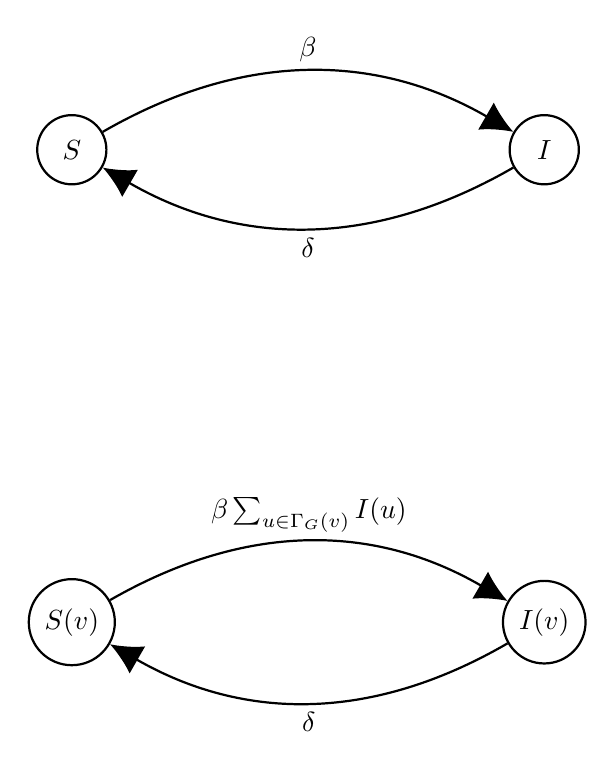
\begin{tikzpicture}[->, auto, thick, node distance=6cm]
	\tikzstyle{every state}=[fill=white, draw=black, thick, text=black, scale=1]

	\node[state] (dumb-S) {$S$};
	\node[state] (dumb-I)[right of=dumb-S] {$I$};

	\path (dumb-S) edge [bend left] node[above] {$\beta$} (dumb-I);
	\path (dumb-I) edge [bend left] node[below] {$\delta$} (dumb-S);
	
    \node[state] (S)[below of=dumb-S] {$S(v)$};
    \node[state] (I)[below of=dumb-I] {$I(v)$};

	\path (S) edge [bend left] node[above] {$\beta \sum_{u \in \Gamma_G(v)} I(u)$} (I);
	\path (I) edge [bend left] node[below] {$\delta$} (S);

	\end{tikzpicture}
        \end{tikzfigure}
    \end{minipage}
  }
\end{columns}

\block{Turning a theorem into a control system}{

  \begin{minipage}[t]{0.5\textwidth}
    \begin{tikzfigure}
      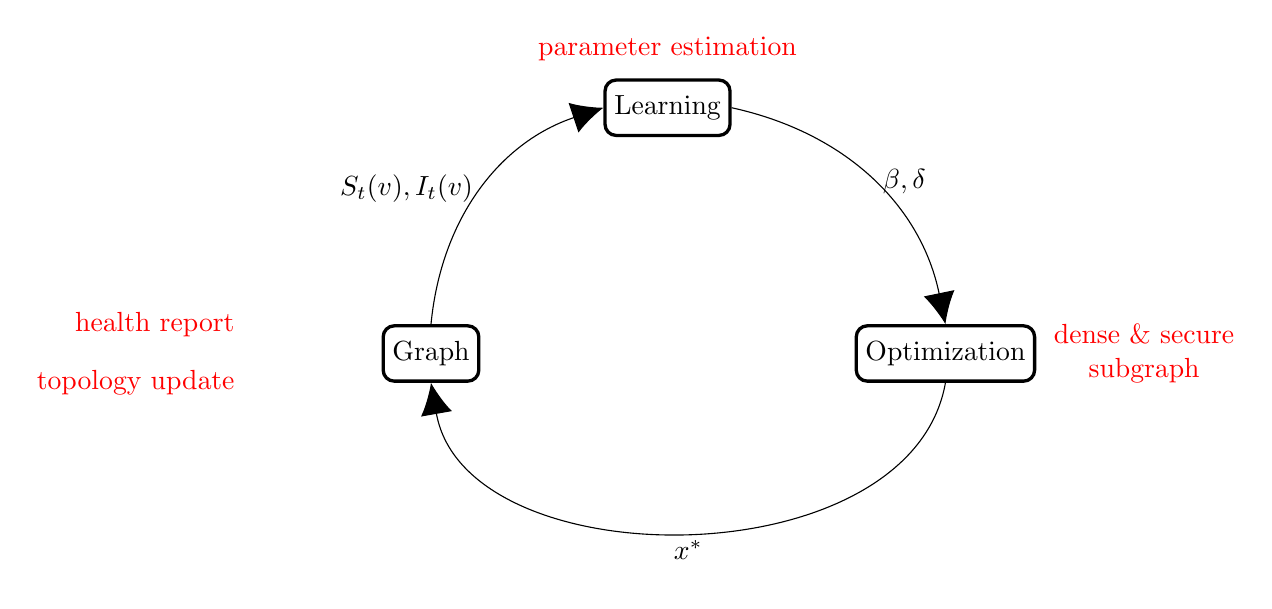
\begin{tikzpicture}[auto, node distance=2.5cm]
      
	\node (control) {};

	\node[rounded-box] (graph) [left=of control.south east] {Graph};
	\node[left=3cm of graph.north east, text=red, align=center] {health report};
	\node[left=3cm of graph.south east, text=red, align=center] {topology update};

	\node[rounded-box] (optimization) [right=of control.south west]  {Optimization};
    \node[right=0.1cm of optimization, text=red, align=center] {dense \& secure\\subgraph};
	
	\node[rounded-box] (learning) [above=of control.north] {Learning};
	\node[above=0.1cm of learning, text=red, align=center] {parameter estimation};

    \path (graph.north) edge [->, bend left=33, align=center] node[left]
        {$S_t(v), I_t(v)$} (learning.west);
	\path (learning.east) edge [->, bend left=33, align=center]
	node[right] {$\beta, \delta$} (optimization.north);
          \path (optimization.south) edge [->, bend left=80] node[below]
          {$x^*$}
		(graph.south);
      \end{tikzpicture}
    \end{tikzfigure}
  \end{minipage}
  \begin{adjustbox}{valign=t}
      \begin{minipage}[t]{0.4\textwidth}

    \begin{Definition}[Spectral radius]
        The spectral radius of a graph is the largest eigenvalue of its
        adjacency matrix and satisfies:
        \begin{equation*}
            \frac{1}{n} \sum_{v\in V} \deg_G(v) \leq \lambda_{\max}(G) \leq
            \max_{v\in V} \deg_G(v).
        \end{equation*}
    \end{Definition}
	\begin{Theorem}[Ganesh et al., 2005]
	  Given a SIS epidemic with parameters $\beta$ and $\delta$ on a graph $G$:
	  \begin{equation*}
          \lambda_{\max}(G) < \frac{\delta}{\beta}
	  \end{equation*}
        implies that the epidemic dies out in time $O(\log n)$.
	\end{Theorem}
      \end{minipage}
  \end{adjustbox}
}

\block{Know your enemy: learning epidemic parameters}{
    \begin{minipage}[t]{0.33\textwidth}
    \subsection*{Anomaly detection}
        \begin{itemize}
            \item[$\circ$] Each node determines its health status by learning.
            \item[$\circ$] One Class SVMs are a family of classifiers used for
                anomaly detection. 
            \item[$\circ$] A OC-SVM is trained on "healthy" data only: the
                system does not require prior experience of the epidemic to
                come. 
        \end{itemize}
    \end{minipage}
    \quad
    \begin{minipage}[t]{0.33\textwidth}
        \subsection*{Maximizing the margin w.r.t. the origin}
        \begin{tikzfigure}
      \begin{tikzpicture}
    \draw [<->,thick] (0,6) node (yaxis) [above] {$y$}
        |- (6,0) node (xaxis) [right] {$x$};
    
	\coordinate (SV1) at (1,4);
	\coordinate (SV2) at (4,1);
    \coordinate (O) at (0,0);
          \node[below left] at (O) {$O$};

          \node[align=center] at (-3, 3) {One Class\\SVM};
    \coordinate (middle-SV) at (2.5, 2.5);

	\draw [brand-orange, thick, shorten >= -0.5cm, shorten <= -0.5cm] (SV1)--(SV2);
    \draw [->, black] (O)--(middle-SV) node [midway, above, sloped] {$w$};
	\fill[brand-orange] (SV1) circle (3pt);
	\fill[brand-orange] (SV2) circle (3pt);

    \coordinate (+1) at (2.3,5.3);
    \coordinate (+2) at (3.5,3);
    \coordinate (+3) at (5.5,2);
    \coordinate (+4) at (3,2.8);
    \coordinate (+5) at (4,5.5);
    \coordinate (+6) at (1.2,5.8);
    \coordinate (+7) at (4.75,4.2);
    \coordinate (+8) at (2,4);
    \coordinate (+9) at (5, 0.5);
    \coordinate (+10) at (1.5,4.1);

    \fill[brand-blue] (+1) circle (3pt);
    \fill[brand-blue] (+2) circle (3pt);
    \fill[brand-blue] (+3) circle (3pt);
    \fill[brand-blue] (+4) circle (3pt);
    \fill[brand-blue] (+5) circle (3pt);
    \fill[brand-blue] (+6) circle (3pt);
    \fill[brand-blue] (+7) circle (3pt);
    \fill[brand-blue] (+8) circle (3pt);
    \fill[brand-blue] (+9) circle (3pt);
    \fill[brand-blue] (+10) circle (3pt);
	  
	\end{tikzpicture}
    \end{tikzfigure}
  \end{minipage}
  \begin{minipage}[t]{0.2\textwidth}
      \subsection*{Parameter estimation}
      \begin{description}
          \item[Input:] Time series of node health data.
        \item[Model:] SIS model with unknown parameters $\beta$ and
            $\delta$.
        \item[Estimate:] $\beta$ and $\delta$.
      \end{description}
  \end{minipage}
}

\block{Approximation algorithms for the secure subgraph problem}{
  \begin{minipage}[t]{0.23\textwidth}
      \subsection*{Closed walks}
      \begin{itemize}
          \item[$\circ$] Norm inequalities give:
              \begin{equation*}
                \lambda_{\max}(A) = O(||A||_{\log n}).
              \end{equation*}
          \item[$\circ$] The number of closed walks of length $k$ is $||A||_k^k$.
          \item Find subgraph with few closed walks of length $\log n$.
      \end{itemize}
  \end{minipage}
  \quad
    \begin{minipage}[t]{0.2\textwidth}
        \subsection*{Mathematical program}
    \begin{equation*}
      \begin{split}
          &\max \sum_{e \in E} x_e\\
          &\sum_{e\in E} x_e A_e \preceq \delta / \beta I\\
          &x \in \{0,1\}^m
      \end{split}
    \end{equation*}
        \begin{itemize}
            \item[$\circ$] $A_e$ is the adjacency matrix of edge $e$.
        \end{itemize}
  \end{minipage}
  \quad
  \begin{minipage}[t]{0.23\textwidth}
      \subsection*{SDP and random matrices}
      \begin{itemize}
          \item[$\circ$] Continuous relaxation of the mathematical program
              gives a SDP.
          \item[$\circ$] Optimal solution $x^*$ used as a distribution.
          \item Leverage concentration of measure for symmetric random matrices.
      \end{itemize}
  \end{minipage}
  \quad
  \begin{minipage}[t]{0.23\textwidth}
      \subsection*{Interlacing polynomials}
      \begin{itemize}
          \item[$\circ$] Polynomial-valued r.v.s related to the
              characteristic polynomial of a graph.
          \item[$\circ$] Undirected graphs have real roots: is it a rare property?
          \item Bounding the spectral radius by bounding roots.
      \end{itemize}
  \end{minipage}
}

\end{document}
